\documentclass[finnish,gradu,twoside,12pt]{tktltiki}

\usepackage[utf8]{inputenc}
\usepackage{natbib}

\usepackage{amsmath}
\usepackage{amsfonts}

\usepackage{graphicx}
\usepackage{hyperref}
\usepackage{rotating}
\usepackage{float}
\usepackage{microtype}

\usepackage{algpseudocode}
\usepackage{algorithm}

\usepackage{listings}
\usepackage{color}

\usepackage{caption}
\usepackage{subcaption}

\usepackage{todonotes}

\begin{document}

%% \onehalfspacing
%\doublespacing

\title{Laskennallinen yhteiskuntatiede politiikan tutkimuksessa}
\author{Matti Nelimarkka}
\date{\today}
\level{LuK --tutkielma}

\numberofpagesinformation{}

\keywords{laskennallinen yhteiskuntatiede, agenttipohjainen mallinnus, ohjattu koneoppiminen, ohjaamaton koneoppiminen}

\maketitle

\begin{abstract}
Tutkielmassa esitellään laskennallisen yhteiskuntatieteen (\textit{computational social science}) käsitettä ja esitellään laskennallisten mentelmien käyttöä politiikan tutkimuksen kirjallisuudessa. Lisäksi valittuja menetelmiä esitellään tarkemmin, jonka jälkeen keskustellaan laskennallisten yhteiskuntatieteiden haasteista tulevaisuudessa.

Kirjallisuuskatsauksen perusteella esitellään politiikan tutkimuksen piirissä käytetyn laskennallinen menetelmä on erilaiset simulaatiomallit, erityisesti agenttipohjaiset simulaatiot nousevat esille käytettynä menetelmänä. Toinen tunnistettu alue laskennallisille menetelmille on teksin analysointi, missä sentimenttianalyysi ja teemojen laskennallinen luokitus nousevat esille.

Systemaattisen kirjallisuuskatsauksen ulkopuolelta nostan esille vielä menetelmiä säännönmukaisuuksien ja ryhmien löytämiseen: assosiaatiosäännöt sekä klusterointialgoritmit. Näitä ohjaamattoman oppimisen menetelmiä ei ole (vielä) sovellettu politiikan tutkimuksen merkittävemmissä lehdissä.

Työn päätteeksi nostan esille laskennallisen yhteiskuntatieteen kaksi haastetta: toisaalta kysymykset liittyen validiteetiin ja reliabiliteettiin ja edelleen haasteet liittyen poikkitieteelliseen työskentelyn. Ensimmäiseen ongelmaan kirjallisuus suosittaa ratkaisuksi laskennallisen tuloksen verifioimista, esimerkiksi vertailemalla tuloksia koeasetelmiin, perinteisin menetelmin saatuihin tuloksiin sekä olemassa oleviin vastaaviin ilmiöihin. Jälkimmäinen ongelma kiteytyy siihen, että tietojenkäsittelytieteilijän ja yhteiskuntatieteilijän tavoitteet ovat erilaiset, eräs ratkaisu tähän voisi olla soveltaa käyttäjäkeskeistä suunnittelua osana laskennallisten mallien kehitystä.
\end{abstract}

\mytableofcontents

\section{Johdanto}

Laskennallisten menetelmien käyttö tutkimusmetelmänä muiden tieteenalojen osana on merkittävä sovellusalue tietojenkäsittelytieteille. Esimerkiksi bioinformatiikka sekä laskennallinen biologia keskittyvät aineiston analyysiin tarvittavien algoritmien ja tiedonlouhinnan kehitykseen. Vastaavasti laskennallisessa kielitieteessä pyritään löytämään laajoista tekstimassoista \textit{(korpuksista)} säännönmukaisuuksia sekä kehittää kuluttajille hyödyllisiä sovelluksia automaattisen kääntämisen piirissä. Opetusalalla tiedonlouhinta mahdollistaa kehittyneempien vuorovaikutteisten sovellusten kehittämisen, kun tiedonlouhinnan avulla mallinnetaan opiskelijan oppimista ja sen muutosta, ja tämän perusteella muutetaan sovelluksien toimintaa. Myös yhteiskuntatieteiden piirissä on herännyt mielenkiintoa soveltaa tietojenkäsittelytieteen menetelmiä ja osaamista tutkimuksen osana, esimerkiksi aineiston käsittelyssä, säännönmukaisuuksien etsimisessä ja yksilön sekä ryhmien toiminnan mallintamisessa.

Viimeaikoina tutkimuskentällä -- varsinkin tietojenkäsittelytieteilijöiden osalta -- on noussut esille suurien tietomassojen käsittely laskennallisesti \textit{(big data analysis)}. Erityisesti viimeaikaisen innostuksen taustalla on niin Internetin kautta \citep{adamic05,notess02} kuin elinympäristöstä kerättyjen aineistojen \citep{eagle06,oulasvirta12} kerääminen sekä tarjoaminen muille tutkijoille. Esimerkiksi sosiologian ja sosiaalipsykologian tutkimuksessa mahdollisuus seurata ihmisten välistä viestintää, sijaintia ja muita tietoja \textit{(reality mining)} mahdollistaa esimerkiksi ystävyyssuhteiden tarkastelun uusilla tavoilla \cite{Karikoski2011a,Nelimarkka2012}. Kuitenkin suurien tietomassojen perusteella tehtävää tutkimusta kohtaan on nostettu esille myös kritiikkiä. Esimerkiksi \citet{Boyd2012a} huomauttavat, että suuret tietomassojen laatu ja hyödyllisyys riippuvat aineistossa käytössä olevista mittareista sekä ympäristön ja taustalla olevien ilmiöiden ymmärtämisestä.

Suurten tietomassojen laskennallinen käsittely on vain osa laskennallisten menetelmien mahdollisista käyttösovelluksista yhteiskuntatieteessä: laskennallisia menetelmiä voidaan käyttää myös perinteisen aineiston käsittelyn tukena ja apuna, käyttäen menetelmiä pienten aineistojen analyysin apuna \citep{pertti}. Yhteiskuntatieteissä, kuten politiikan tutkimuksessa, käsitellään useita erilaisia tutkimuskysymyksiä joihin on mahdollista vastata laskennallisesti. Laskennallisten menetelmien mielenkiintoisuutta voidaan perustella kahdella eri syyllä

\begin{enumerate}
\item laskennalliset menetelmät mahdollistavatuusien menetelmien käytön ja mahdollistavat näin  \textit{uudenlaisten kysymysten} kysymisen
\item laskennalliset menetelmät \textit{tehostavat} aineiston käsittelyä ja näin esimerkiksi vähentävät tarvetta manuaaliselle työlle
\end{enumerate}

Erityisesti mielenkiintoisuutta nyt lisää se, että tietotekniikka on jokapäiväistynyt ja laskennallisten menetelmien soveltaminen on yleistynyt muiden tieteiden parissa. Laskennallisten menetelmien soveltaminen on myös nousemassa oleva trendi yhteiskuntatieteissä, osittain työtä tehdään tietojenkäsittelytieteen puolelta -- mutta enevemissä määrin myös yhteiskuntatieteilijät soveltavat laskennallisia menetelmiä. Tarpeen onkin pyrkiä esittelemään laskennallisia menetelmiä ymmärrettävästi myös suomen kielellä.

Kirjallisuuden rajaamiseksi tässä työssä yhteiskuntatieteiden osalta keskitytään politiikan tutkimukseen. Ennen tarkempaa paneutumista laskennallisuuteen ja tietojenkäsittelytieteeseen on tarpeen esittää politiikan tutkimuksen oppihistoriaa ja nykyisin vakiintuneita menetelmiä lyhyesti, jolloin laskennalliset menetelmät voidaan sijoittaa osaksi politiikan tutkimuksen traditiota. Tämän jälkeen esitellään olemassa olevia määritelmiä laskennalliselle yhteiskuntatieteelle ja esitellään kirjallisuuskatsauksen tuloksia laskennallisten menetelmien käytöstä yhteiskuntatieteissä. Kolme menetelmäryhmää esitellään tarkemmin niin sovellutusten kuin laskennan pohjalta: simulaatiot, tekstianalyysi ja säännönmukaisuuksien etsiminen. Kirjallisuuskatsauksen perusteella keskustellaan laskennallisen yhteiskuntatieteen haasteista.

%% Tällöin perinteiset ei-laskennalliset menetelmät eivät välttämättä sovellu tutkimukseen, ja samaan aikaan laajat aineistot mahdollistavat aiemmin haastavina pidettyjen menetelmien käytön -- esimerkiksi verkosto-analyysin ongelma on ollut aineiston vaikea keräys \citep{a}. Tällöin myös rahoittajien korostama poikkitieteellinen lähestymistapa \citep[60]{tieteentila12} on ensinnäkin mahdollinen resurssien myötä ja toisaalta välttämätön, koska perinteiset lähestymistavat eivät käytä hyödykseen mahdollisuuksia joita laskennallisten tieteiden kehitys on luonut.

\subsection{Politiikan tutkimuksen oppihistoriaa}

%% Työssä esitetään laskennallisia menetelmiä joita sovelletaan yhteiskuntaa koskeviin kysymyksiin vastaamiseksi: laskennallisen yhteiskuntatieteen malleihin, sovelluksiin sekä tieteenfilosofiaan. Työssä yhteiskuntatiede nähdään laajasti yhteiskuntaa tutkivien tieteiden joukkona, joihin kuuluvat esimerkiksi politiikan tutkimus, taloustiede, sosiologia, sosiaalipyskologia ja viestinnän tutkimus\footnote{Tässä työssä esimerkit on erityisesti valittu politiikan tukimuksen näkökulmasta, mutta esitetyt menetelmät ovat laajemmin sovellettavissa laajemminkin yhteiskuntatieteisiin.}. Tutkimusaloille tyypillistä on samankaltaisten tutkimuskysymysten lähestyminen kunkin alan oman oppihistorian sekä käsitteistön kautta \citep{a}. Esimerkiksi poliitikkojen sosiaalisen median käyttöä voidaan lähestyä niin politiikan tutkimuksen, viestinnän tutkimuksen kuin esimerkiksi sosiologian näkökulmasta. Esimerkki.

%% Kuten yllä olevista esimerkeistä huomataan, eri yhteiskuntatieteet käsittelevät samankaltaisia kysymyksiä, kuitenkin erilaisin painotuksin. Nykyinen eriytyminen eri tieteenaloihin on osa tieteenalan laajempaa kehittymistä nykyiseen käsitykseen yhteiskuntatieteestä. Jotta yhteiskuntatieteen nykyinen tila, sen puutteet ja laskennallisten menetelmien tarjoamat mahdollisuudet ymmärrettäisiin, niin on tarpeen esitellä yhteiskuntatieteen oppihistoriaa tiiviisti. Eräs merkittävä muutos joka valtavirran tutkimuksessa sijoittuu 1950 -- 1960-luvuille on behavioralismin vaikutus yhteiskuntatieteisiin. Ennen tätä muutosta yhteiskuntatieteet, varsinkin 1800-luvun lopussa sekä 1900-luvun alussa, olivat kuvailevia ja normatiivisia: erilaisia havaintoja kuvailtiin varsin laajasti \citep{x} ja yhteiskuntafilosofia\footnote{Jonka historia toki on merkittävästi laajempi, esimerkiksi Platonin Valtio voidaan nähdä yhteiskuntaa kuvaavana filosofiana ja Hobbesin sekä Locken sopimusteoriamallien kautta muodostetut käsitteellistykset valtiosta toimijana ovat hyviä esimerkkejä perinteisestä normatiivisesta ajattelusta} oli yhteiskuntatieteen keskeistä sisältöä. Kuitenkin, behavioralismin myötä käänne empiiriseen tutkimukseen, todellisten ilmiöiden havainnointiin ja niiden arviointiin, oli merkittävä. Tätä siirtymää kuvaa \citep[yy]{x} kuvaus yhteiskuntatieteestä:


Politiikan tutkimuksen ensimmäiset teemat keskittyivät historialliseen sekä normatiiviseen tutkimukseen, esimerkiksi aatehistorian sekä käsitteiden määrittelyyn. Politiikan tutkimuksen toinen vaihe 1900--luvun alussa kehitti lähestymistapoja empiirisemmäksi ja tutkimusmenetelmissä pyrittiin lähestymään luonnontieteitä \citep{historia}. Edelleen, menetelmien lisäksi tutkimuskysymykset muuttuivat tutkimaan ihmisten toimintaa ja käyttäytymistä, jonka takia tästä komannesta vaiheesta käytetään nimeä \textit{behavioralismi}.

Behavioralismi myös esitti oletuksia ihmisten käyttäytymisestä, joka yhdistettynä luonnontieteelliseen toimintatapaan johdatti politiikan tutkimuksen kohti erilaisten mittareiden kehitystä ja muuttujien operationalisointia. Behavioralistinen tutkimus voisi siis soveltaa laskennallisen tieteen menetelmiä: esimerkiksi peliteoria ja sen sovellukset olivat tyypillisiä menetelmiä mallintaa ilmiöitä, ja näiden ajatusmallien siirto laskennalliseen muotoon on mahdollista, ja jopa mielekästä.

Tämä nosti esille vastaliikkeitä, joita yhdessä kuvataan termillä kriittinen koulukunta. Kriittisen koulukunnan mukaan yhteiskunnan tutkimuksessa on tarpeen laajempi näkökulma teemoihin. Samoin kriittinen koulukunta kyseenalaisti behavioralismin objektiivisuuden, argumentoiden, että tutkimuksen operationalisoinnit luovat jo subjektiivisen ulottuvuuden ja tulosten tulkinta on edelleen subjektiivista. Tietenkin, myös kriittisen koulukunnan työskentelyä kuvaa subjektiivisuuden keskeinen luonne tutkimuksen osana -- mutta, tämä subjektiivisuus onkin usein osa kaikkea yhteiskuntatiedettä. Subjektiivisuuden kehitys osaksi laskennallisia malleja voi kuitenkin olla haastavaa, vaikkei mahdotonta.

\begin{figure}
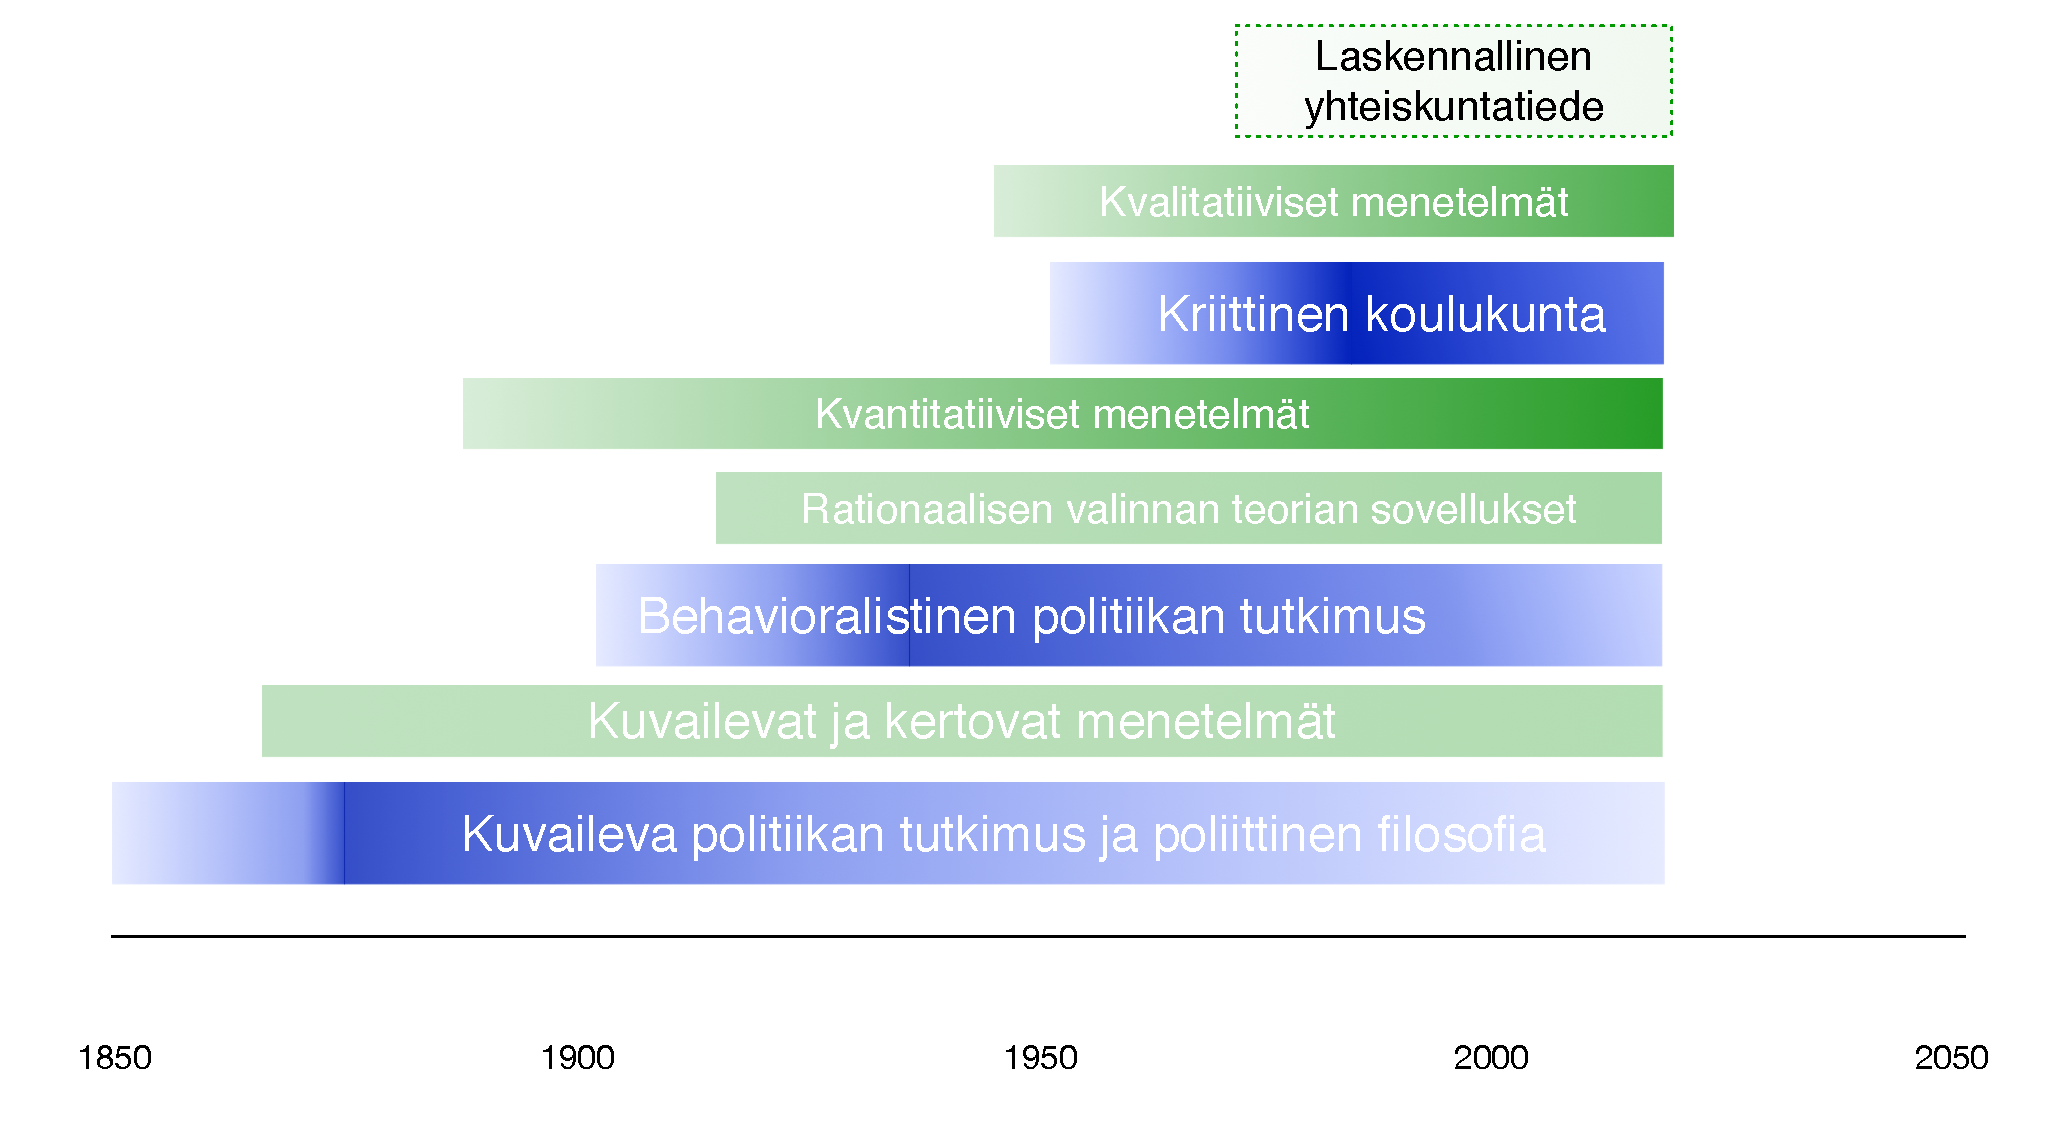
\includegraphics[width=12cm]{images/historia.pdf} 
\caption{Politiikan tutkimuksen oppihistoriaa tiivistetysti}
\label{fig:historia}
\end{figure}

Yksinkertaistetusti politiikan tutkimuksen historia voidaan esittää kolmen vaiheen kautta, kuten kuvassa \ref{fig:historia} on tehty. Vaihteet ovat liittyneet myös menetelmäkehitykseen, joka on liitetty osaksi alan oppihistoriaa kuvassa. Modernissa empiirisessä yhteiskuntatieteesä voidaan siis nostaa esille kahden laajemman lähestymistavan soveltaminen tutkimuskysymyksiin. Tutkimuksessa sovelletaan yleensä laadullista (kvalitatiivinen) tai määrällistä (kvantitatiivinen) tutkimusotetta, missä ensimmäisessä pääpaino on enemmän kuvailevassa aineistossa ja sen tulkinnassa, jälkimmäinen taas pyrkii mitattaviin aineistoihin ja selittämiseen matemaattisia menetelmiä hyödyntäen. Sellaisenaan voimakasta menetelmäjakoa on kritisoitu, koska useiden ilmiöiden kohdalla olisi mielekästä soveltaa molempia tutkimusmenetelmiä: laadullisen tutkimuksen perinteinen haaste on tutkimuksen yleistettävyys koko joukkoon, kun taas määrällisen tutkimuksen tapauksessa kausaalisen tekijän keskeinen luonne voi helposti jäädä selvittämättä \citep{ragin96,mcgraw96,silverman00}.

Kritiikkini kausaalisuuden puutteesta voi olla yllättävä, joten valaistaan tilannetta esimerkillä: on havaittu, että poliitikot eivät suosi vuorovaikutuksellista ja kaksisuuntaista verkkomedian käyttöä, vaan käyttävät verkkomediaa perinteisen median jatkona \citep{Golbeck2010}. Kuitenkaan, nämä määrällistä lähestymistapaa soveltavat tutkimukset eivät täysin pysty selittämään miksi näin on. Tällöin on tarve laadulliselle tutkimukselle, kuten \citet{Stromer-Galley2000} havannointityölle ehdokkainen parissa, missä hän esittää, että ehdokkaat pelkäävät interaktiivisen viestinnän altistavan heidät kyseenalaistamiselle ja mahdollisesti sotkevan kampanjaviestintää. Näin vakuuttavaan yhteiskuntatieteelliseen argumentaatioon vaaditaan toisaalta määrällistä, koko tutkittavan joukon kattavaa havaintoa sekä laadullista työskentelyä, mikä joko selvittää havaintoja -- kuten yllä -- tai nostaa esille uusia tutkimuskysymyksiä.

\subsection{Laskennallinen yhteiskuntatiede}

Määrällisestä lähestymistapaa edustavat tilastollisten menetelmien soveltaminen aineiston käsittelyssä, mutta myös formaalit menetelmät, kuten peliteoria voidaan laskea osaksi tätä lähestymistapaa. Myös tarkastelun kohteena oleva laskennallinen yhteiskuntatiede (\textit{computational social science}) edustaa määrällistä lähestymistapaa, mikä on ilmeistä kirjallisuudessa esitettyjen laskennallisten yhteiskuntatieteiden määritelmistä:

\begin{description}
\item[\citet{cioffi-revilla10}] määrittelee laskennallisen yhteiskuntatieteen laajasti seuraavien laskennallisten menetelmien soveltamisena: tiedon uuttamisen menetelmät (\textit{information extraction}), sosiaalisten verkostojen analyysi, paikkatietojärjestelmien käyttämisen ja mallinnuksen sekä simulaation menetelmät. Hän myös arvioi, että tiedon visualisointimenetelmät voivat myöhemmin laajentua käytettäväksi laskennallisen yhteiskuntatieteen menetelmänä. Hän siis näkee, että laskennallista tiedettä voidaan määritellä tiettyjen menetelmien käyttönä.
\item[\citet{lazer09}] taas esittää laskennallisen yhteiskuntatieteen laajojen aineistomäärien keräämisenä ja käsitttelynä määrällisten menetelmien avulla. He nostavat esille, että laskennallinen yhteiskuntatiede on aineistolähtöistä (\textit{data-driven}), minkä tulkitsen tarkoittavan, että perinteinen hypoteeseihin ja niiden tarkasteluun perustuvat tilastolliset menetelmät eivät olisi laskennallista yhteiskuntatiedettä.
\item[\cite{bankes02}] kuvaavat laskennallisia epistemologioita (\textit{computational epistemology}), eli käsityksiä hyvästä tieteestä. Toisaalta he ehdottavat, että laskennallinen yhteiskuntatieteen tarkoitus on luoda selittäviä malleja, joiden avulla yhteisöä voidaan tutkia. Toisaalta, he nostavat esille myös mahdollisuuden käyttää näitä malleja ei vain yhteisön tutkimiseen vaan myös laskennallisten koeasetelmien suorittamiseen. Tässä määritelmässä siis tärkeintä on tutkittavan ilmiön mallinnus laskennallisin menetelmin.
\end{description}

Kuten havaitaan, laskennallisten menetelmien käsitteet eivät ole kaikilla tutkijoilla samankaltaisia, johtuen myös erilaista lähestymistavoista laskennallisen yhteiskuntatieteen määritelmään. Kuten \citet{cioffi-revilla10} huomauttaa, laskennallisen tieteen osalta voidaan erottaa laskennallisuus menetelmänä ja laskenta teoreettisena lähtökohtana. Jaottelu ei kuitenkään ole ongelmaton: esimerkiksi nykyisin tilastollisten menetelmien kohdalla käytetään poikkeuksetta laskennallista välineistöä. Toisaalta, sosiaalisen verkostojen analyysin kohdalla taustalla on graafiteoria ja sen sovellukset, vaikkakin niitä suoritetaan laskennallisesti. Tässä työssä on syytä esittää tarkempi rajaus laskennallisen yhteiskuntatieteen toimintakentästä, koska rajaus vaikuttaa käsiteltäviin aiheisiin.

\subsection{Kirjallisuuskatsaus}

Havaitaksemme kuinka erilaisia laskennallisten menetelmien käytetään yhteiskuntatieteissä suoritan kirjallisuuskatsauksen laskennallisten mentelmien käytöstä politiikan tutkimuksessa. Etsin kirjallisuuskatsauksessa termejä ``computational social science``, ``machine learning``, `ìnformation extraction``, ``simulation` sekä ``data-mining` artikkeleista käyttäen Web of Science --tietokantaa. Politiikan tutkimuksessa erittäin arvostetut lehdet ovat American Political Science Review (APSR), American Journal of Political Science  (AJPS), Annual Review of Political Science (ARPS), Comparative Political Studies (CPS) sekä European Journal of Political Research (EJPR). Tietokanta sisälsi APSRn numerosta 50 lähtien (vuodesta 1956), AJPSn numerosta 17 (1973), ARPSn sekä CPSn ensimmäisestä numerosta (1998, 1968) ja EJPRn numerosta kolme (1975). Tietokannassa olevat artikkelit olivat julkaistu toukokuuhun 2014 mennessä. %% Political Studies (PS) sekä Political and Society (P\&S).

Löydettyjen artikkelien on esitetty taulukossa \ref{kirjallisuuskataus}, josta havaitaan ettei laskennallisia menetelmiä käytetä vielä alan merkittävimmissä lehdissä, poikkeuksena simulaatiotutkimukset. Simulaatioon liittyviä 46 artikkelia tarkasteltiin tarkemmin niiden abstraktin pohjalta, jonka perusteella simulaatiotiotutkimukset voidaan jakaa neljään perheeseen: simulaatiot aineiston luomisessa tai tilastollisesessa testauksessa, agenttipohjaiset mallit, Monte Carlo --pohjaiset mallit sekä tapauskohtaiset erityismallit. Kappaleessa \ref{simulaatio} esitellään simulaatiomenetelmiin liittyviä tuloksia ja käytettäviä menetelmiä tarkemmin.

\begin{table}

\begin{tabular}{lrrrrr}
~  & CSS & ML & IE  & SIM & DM \\
\hline
APSR  & 0 & 0 & 0 & 20 & 0 \\
AJPS  & 0 & 0 & 0 & 21 & 0 \\
ARPS  & 0 & 0 & 0 &  1 & 0 \\ 
CPS   & 0 & 0 & 0 &  2 & 0 \\
EJPR  & 0 & 0 & 0 &  2 & 0 \\
\hline
%% PS    & 15  & 243 & 41 & 86  & 172 \\
%% P\&S  & 4   & 63  & 0  & 12  & 76  \\
SSCR & 12 & 3 & 0 & 46 & 4  \\
\hline
\end{tabular}
\caption{Hakuosumat kirjallisuudesta}
CSS = Computational Social Science, ML = Machine Learning, IE = Information Extraction, SIM = Simulation, DM = Data Mining
\label{kirjallisuuskataus}

\end{table}

Koska käytössä olleet menetelmät olivat varsin vähäiset suhteessa yllä esitettyihin, varsin laajoihin kuvauksiin laskennallisesta yhteiskuntatieteestä, on syytä tarkastella muitakin julkaisuja, erityisesti Social Science Computer Review:tä (SSCR)\footnote{Saatavilla numerosta kahdeksan, vuodesta 1990.} tietojenkäsittelytieteen ja yhteiskuntatieteen yhteisenä lehtenä. Vaikkei kyseessä ole erityisesti politiikan tutkimuksen lehti, lehden menetelmät ovat sovellettavissa myös politiikan tutkimukseen. Edelleen simulaatiomallien määrä suhteissa muihin menetelmiin on suurehko, mutta erityisalan lehdessä on edustettuina myös muita laskennallisen yhteiskuntatieteen töitä. Jälleen simulaatioiden käyttö on yleisin käytössä oleva menetelmä, tiedon louhinna teemana alla nostetaan esille erilaisia menetelmiä tekstiaineistojen analysoimiseksi, näitä käsitellään tarkemmin kappaleessa \ref{sec:textanalysis}.

Lisäksi kappaleessa \ref{unsupervised} nostetaan esille ohjaamattoman oppimisen \textit{(unsupervised learning)} menetelmiä, joita on havaittu kirjallisuuskatsauksen ulkopuolisessa kansainvälisessä vertaisarvioidussa kirjallisuudessa kahden vuoden seurannan aikana. Nostan esille esitettyjä menetelmiä uusina avauksina, joita voitaisiin laskennallisessa yhteiskuntatieteessä soveltaa laajemminkin, vaikkei ne nyt suoritetussa kirjallisuuskatsauksessa nousseet selkeästi esille.

%% On myös syytä perustella tutkimusaiheen relevanttius sekä yhteiskuntatieteellisen että teknillistieteellisen näkökulman kautta. Eräs syy laskennallisten menetelmien yleistymiseen on laskennan resurssien saavutettavuus \cite{z,x}, minkä johdosta erilaisia menetelmiä nostetaan esille usein. Uudet laajat tietovarastot, niin

\section{Simulaatiot ilmiöiden tarkastelussa}
\label{simulaatio}

% Yhteiskuntatieteissä simulaatiopohjaista mallinnusta on sovellettu tarkastellessa yhteisöjen toimintaa ja niiden rakentumista \citep[esimerkiksi][]{Epstein2002a,Epstein2001,Cederman2003,Villatoro2013} kuin organisaation toimintaa \citep[esimerkiksi][]{VonRandow2011,Pearson2011}. Perustana on ajatus, että yksittäisten toimijoiden päätökset vaikuttavat kokonaisuutena yhteiskunnan rakenteisiin -- erityisesti tarkastelemalla joukon heterogeenisyyttä sekä sosiaalisen vuorovaikutuksen merkitystä \citep{Squazzoni2013}.

% \citet{Epstein2002a} mallintaa kansalaistottelemattomuuden muutosta poliisien ja aktivistien suhteen. Aktivistit reagoivat legimiteetin ja kokemansa vaikeuden (\textit{hardship}) muutokseen: vähäisempi legitimiteetti ja suurempi koettu vaikeus johtavat radikalisoitumiseen. Lisäksi mallissa muutetaan agenttien liikkumista, poliisien määrää ja poliisien vangitsemien aktivistien vankilassa pitämää aikaa. Eri arvojen pohjalta suoritetaan kahdeksan ajoa, joiden pohjalta tarkastellaan yhteiskunnan tilaa. Erilaisten ajojen määrä tässä julkaisussa on siis varsin vähäinen, mikä osittain kyseenalaistaa havaittuja tuloksia -- jotka kuitenkin perustuvat sattumaan\footnote{Esimerkiksi \citet{Dragicevic2014} esittelevät, kuinka tilastollisesti merkittävät erot voivat aiheutua pienistä muutoksista simulaatiossa.}. Lisäksi mallin pohjalta tarkastellaan esimerkiksi legitimiteetin ja poliisien määrän muutosten vaikutusta yhteiskuntaan.

% Edelleen \citet{Epstein2001} arvio sosiaalisten normien kehittymistä määrittelemällä kullekkin agentille ensisijaisen normin sekä tarkkailuetäisyys, jonka perusteella agentti mukauttaa omaa normiaan muiden normeihin. Kyseessä siis on sosiaalisoitumisprosessin simulointi laskennallisesti. Jälleen mallien parametreja muutetaan, jotta voidaan havaita erilaisia yhteiskunnallisia tilanteita ja sääntöjen vaikutusta lopputuloksiin; kutakin parametria kuitenkin simuloidaan vain kerran. Myös \cite{Villatoro2013} paneutuvat normien toimintaan simuloinnissan, tarkkailen rankaisun merkitystä normien syntymisessä ja ylläpitämisessä. Työn voi myös tulkita edustavan modernimpaa simulaatiotutkimusta: simulaatiota on toistettu 5000 kertaa tulosten vahvistamiseksi, ja simulaatioaineiston saatavuus on erikseen mainittu artikkelissa.

% Yhteiskuntatieteellisten teorioiden lisäksi agenttipohjaisen simulaation sovelluskohteena on ollut erityisesti julkisten organisaatioiden toiminta ja sen kehittäminen. Esimerkiksi \citet{Pearson2011,VonRandow2011} arvioivat vanhustenhoidon tulevia tarpeita simulaatiomallin pohjalta. Kyseessä on mikrosimulaatiomalli, jolloin mallin taustaoletukset perustuvat saatavissa oleviin tietoihin, toisin kuin agenttipohjaisissa malleissa -- missä parametrien arvojen valinta on ollut mielivaltaista.

%% Yllä käsiteltiin sosiaalisen prosessin tutkimusta, eräs varhainen -- ei laskennallinen vaan behavioralistiseen koulukuntaan -- kuuluva tutkimus on  \citet{Granovetter1978} yhteisön toimintaa ja sen käynnistymistä käsittelevä tutkimus.

%% A comparison of agent-based models of income tax evasion

Kirjallisuuskatsauksen pohjalta simulaatiopohjaiset tutkimukset voitiin jakaa neljään ryhmään: simulointi tilastotieteen välineenä \citep[esimerkiksi][]{clinton2004statistical,imai2012statistical,mooney1996bootstrap,slantchev2004initiators}, toimialakohtaiset mallit ja niiden simulointi \citep[esimerkiksi][]{Shapiro1968} sekä agenttipohjaiset mallit \citep[esimerkiksi][]{orbell2004machiavellian,altaweel2012mobilizing,anderson2011highlights,bloomquist2006comparison}. %% ja Monte Carlo --simulointi \citep{quinn1999voter,jackman2000estimation,}.

Laskennallisen yhteiskuntatieteen kannalta tilastollinen simulointi, esimerkiksi bootsrap-menetelmien käyttö, ei ole mielenkiintoista. Myös toimialakohtaisiin malleihin perustuva simulointi on vanhempaa tutkimusta: esimerkiksi \citet{Shapiro1968} on työssään rakentanut mallin siitä, kuinka Yhdysvaltojen edustajainhuone äänesti vuosina 1963--1964, ja arvio mallin toimintaa suhteissa aitoihin äänestyspäätöksiin. Kuvassa \ref{fig:domain_sim} nähdään osa simulaatiomallia. Kyseessä on varsin laaja, mutta yksinkertainen, algoritmi arvioimaan sosiaalisen vuorovaikutuksen merkitystä päätöksentekotilanteessa. Merkittävä ero nykyisiin simulaatiomalleihin on niiden yksinkertaisuus: kullekkin toimijalle luvut ovat samat, eikä satunnaistekijöitä ole mukana mallissa. Tämän yksinkertaisuuden takia nämä mallit eivät ole mielenkiintoisia laskennallisen yhteiskuntatieteen piirissä.

\begin{figure}
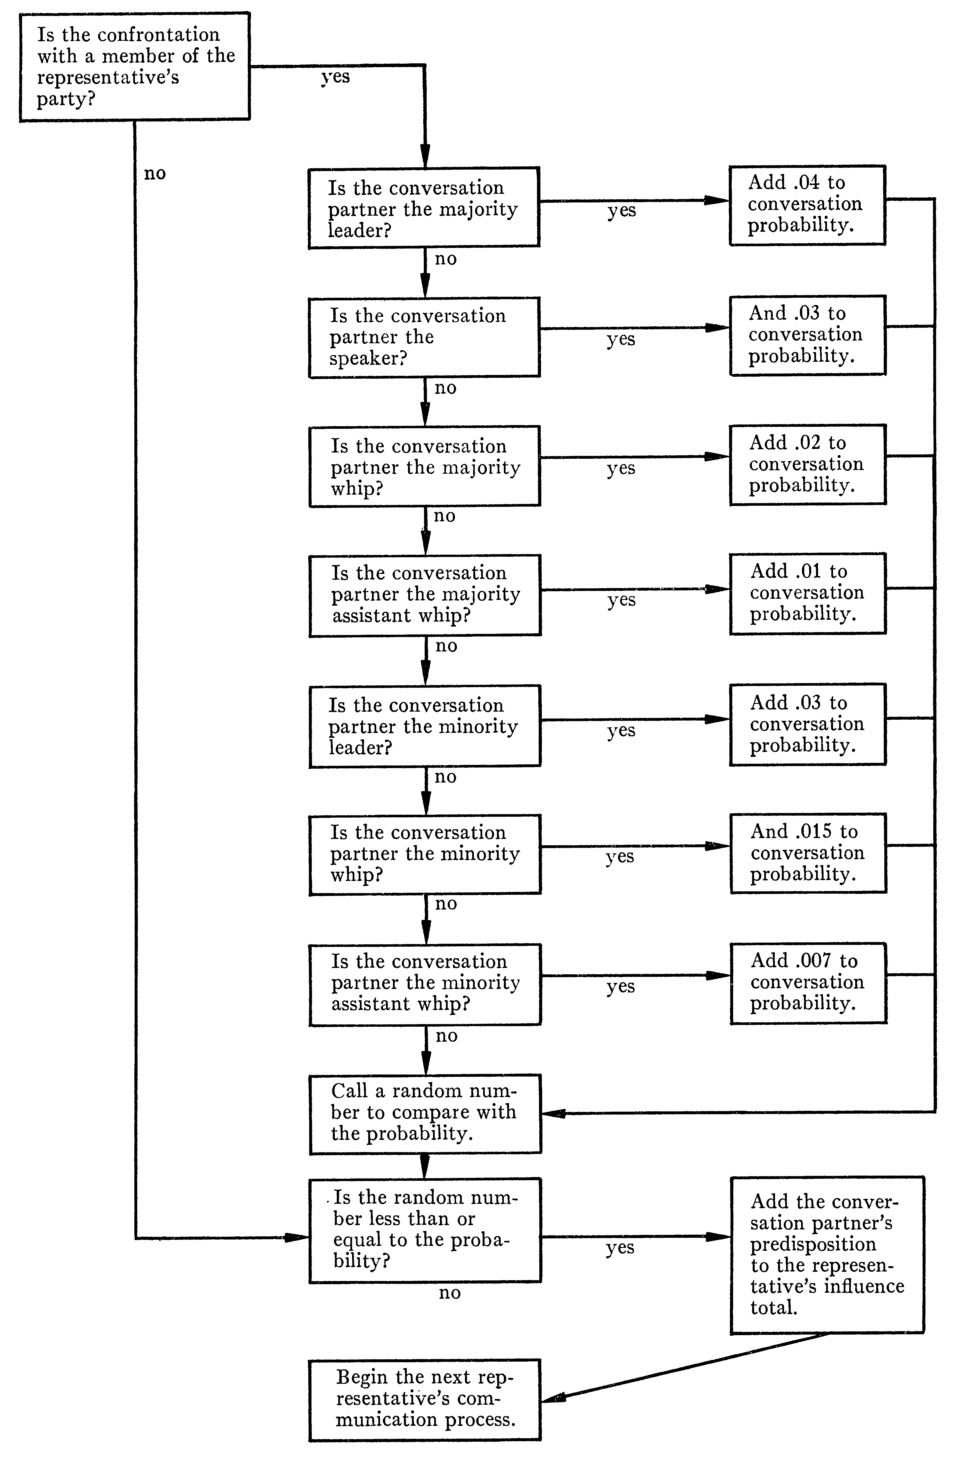
\includegraphics[height=10cm]{images/domain_spesific_model.png} 
\caption{Toimialakohtaisen mallin simulaation eräs osa \citep{Shapiro1968}}
\label{fig:domain_sim}
\end{figure}

Uudempi simulaatioperinne ottaa paremmin huomioon niin erilaisten toimijoiden kuin satunnaisuuden roolia. Esimerkiksi \citet{orbell2004machiavellian} arvioivat yhteistyöhön liittyvien normien kehittymistä useiden vuosisatojen aikana simuloiden normeja ja niiden vaikutusta yhteiskunnassa. Mallin perusteella Orbell et al. argumentoivat, että yhteistyön tapahtumista tukee mahdollisuus arvioida toisen toimijan tilannekuvaa ja motiiveja. Myös \citet{altaweel2012mobilizing} käyttävät agenttipohjasta simulointia poliittisten protestien simulointiin ja esittävät mallissaan arvioita erilaisten tekijöiden, kuten rahoituksen ja rangaistusten vaikutusta protestiliikkeiden muodostumisessa. Yllättävää kyllä, kummassakin tapauksessa mallin pohjalta tehtiin varsin vähän ajoja, jolloin mallien satunnaistekijät eivät välttämättä nouse luotettavasti esille. Kuitenkin, muten \citet{Villatoro2013} ovat tehneet, simulaatiota voidaan ajaa usempia kertoja -- heidän tapauksessaan 5000 kertaa -- tulosten vahvistamiseksi ja simulaation pohjalta muodostettu aineisto on myös luvattu, avoimen tieteen hengessä, tutkijoiden käyttöön. Heidänkin työnsä tarkastelee rankaisun merkitystä normien synnyssä ja ylläpitämisessä. Laajojen yhteiskunnallisten ilmiöiden simuloinnin lisäksi menetelmiä voidaan käyttää niin sairaalan organisaation ja kansanterveystyön ennustamiseen \citep{Pearson2011} kuin myös veropäätösten vaikutukseen arviointiin \citep{bloomquist2006comparison}.

%% Agenttipohjaisen mallinnuksen lisäksi satunnaistekijöitä voidaan huomioida Monte Carlo--simuloinnilla -- jolloin ei niinkään mallinneta yksittäisen agentin toimintaa ja vuorovaikutusta vaan käytetään yksinkertaisempaa mallia ilmiöstä, esimerkiksi Sovelluskohteina on ollut esimerkiksi äänestyspäätökset \citep{quinn1999voter,jackman2000estimation} sekä sodan päättymisen ennustaminen \citep{slantchev2004initiators}.
 
\subsection{Agenttipohjainen malli}

\begin{figure}
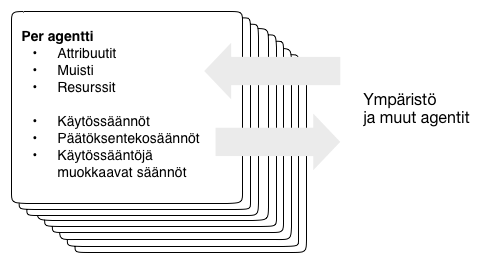
\includegraphics[height=6cm]{images/agenttimalli.png} 
\caption{Agenttipohjainen simulaatio \citet{Macal2009} mukaan}
\end{figure}

Agenttipohjaisesissa malleissa (\textit{agent-based models, ABM}) mallinnetaan yhteisön toimintaa yksittäisten toimijoiden kautta. Kukin toimija, eli agentti, on yksilöllinen toimintaheuristiikka, tai prefrenssifunktio. Tämän preferenssifunktion sekä mahdollisen satunnaisfuntion avulla määritellään agentin tila seuraavalla ajanhetkellä: \begin{equation}\mathcal{T}_{i,(t+1)} = \mathcal{P}( \mathcal{T}_{i,t} ) + \varepsilon \label{abm:yhtälö}\end{equation} Toistamalla sama simulaatio järjestelmän kaikille agenteille, voidaan määrittää järjestelmän tila ajanhetkellä $t+1$ ajanhetken $t$ perusteella. Luonnollisesti preferenssifuntio $\mathcal{P}$ voi ottaa huomioon myös muiden agenttien toimeinpiteet ja tästä syntyneen järjestelmän tilan tehdessään päätöstä tulevasta tilasta \citep[esimerkiksi][]{Bonabeau2002}. Mallinnusprosessia siis joudutaan etukäteen määrittelemään merkittäviä muuttujia, joka \citet{Gilbert1993} mukaan helpottaa teorioiden muodostamista ja testaamista: simuloidussa malleissa kun ei voida ottaa huomioon kaikki yhteiskunnallista ilmiötä kuvaavia muuttujia.

\citet{Bonabeau2002} kuvaa tarkemmin agenttipohjaisen mallien hyötyjä. Hänen mukaansa agenttipohjainen mallinnus havaitsee paremmin nousevia ilmiöitä {\textit{emergent phenomena}), eli ilmiöitä joita ei voida havaita tarkastellessa vain yksilöitä, vaan yksilöiden välinen vuorovaikutus tai toisten yksilöiden toiminta vaikuttaa yksilön käyttäytymiseen. Esimerkkeinä täläisistä tilanteista on oppiminen ja sopeutuminen (ajallinen korrelaatio), aikaisempi kokemus ja tehdyt päätökset (muisti sekä polkuriippuvuus) sekä epälineaarinen käyttäytyminen, esimerkiksi tietyn kynnysarvon jälkeen tapahtuva toiminta.

Toisena hyötynä \citet{Bonabeau2002} mainitsee agenttipohjaisen mallin helpomman tulkittavuuden. Hän arvioi, että yksilökeskeinen kuvaus toiminnasta on selkeämpi kuin erilaiset tilasiirtymäkuvaukset tai prosessikuvaukset. Tämän takia hän arvioi agenttiohjaisen mallien olevan helpommin asiantuntijoiden tulkittavissa ja arvioitavissa, jolloin mallit ovat selkeämmin validoitavissa. Lisäksi \citet{Bonabeau2002} kritisoi keskisuureiden käyttämistä ilmöiden kuvaamiseksi, koska näissä tilanteissa ääriarvot eivät ole nähtävissä ja keskisuureet tasoittavat vaihtelua.

\subsection{Mikrosimulaatiot}

Agenttipohjaisten mallien lisäksi on mahdollista käyttää mikrosimulaatiota  (\textit{microsimulation model}). Sen toiminta ei merkittävästi eroa esitetystä yhtälöstä \ref{abm:yhtälö}, eli malli pyrkii ennustamaan yksilön toimintaa. Kuitenkin taustalla oleva lähestymistapa eroaa. Agenttipohjaisen malli pyrkii luomaan ilmiön parametrien avulla ja tämän jälkeen tarkastelemaan luomiseen tarvittuja parametreja, kun taas mikrosimulaatiossa ilmiöön liittyvät taustamuuttujat ja niiden väliset määritellään etukäteen \citep[58--59]{Gilbert2005}. Yksilökeskeisen mallinnustavan takia pidän mikrosimulaatioita ja agenttipohjaisia malleja samankaltaisina agenttipohjaisina simulaatioina, vaikka niiden toiminnan yksityiskohdat eroavatkin toisistaan.

\subsection{Tit for tat}

Kirjallisuuskatsauksessa ei esiintynyt erästä agenttipohjaisen simulaation varianttia, jossa mallinnetaan erilaisia käyttätysmismalleja ja niiden vaikutusta lopputulokseen. Alan klassikko on \citet{Axelrod01031980} simulaatio yhteistoiminnasta, nimenomaisesti siitä kuinka agenttien kannattaa rankaista toisiaan sääntöjen rikkomisesta. Mallinnus perustui rationaalisen valinnan olettamuksiin yksilöistä oman edun edun tavoittelijoina ja koko asetelman pohjalla onkin peliteorian soveltaminen vuorovaikutuksen analyysiin.

\citet{Axelrod01031980} esittelee kilpailua, jossa etsittiin simuloimalla voittavaa strategiaa vangin dilemma-tyyppisessä asetelmassa, jossa yhteistyöstä palkitaan molempia pelaajia, mutta jos pelaaja pettää -- ja on ainoa pettäjä -- palkinto on suurempi kuin yhteistyössä. Molempien pettäessä kumpikaan pelaaja ei saanut palkintoa. Kilpailun voittanut strategia oli yksinkertaisin: petä jos aiemmalla kierroksella sinua on petetty, muutoin toimi yhteistyön mukaisesti. Tuloksen sovelluksia on ollut erityisesti kansainvälisten suhteiden alalla.

\subsection*{Kirjastot ja kehitysympäristöt}

Agenttipohjaisen simulaation toteutukseen on olemassa useita erilaisia valmiita kirjastoja sekä alustoja. \cite{Tobias2004} esittää arviointikriteereitä onnistuneille simulaatioympäristöille: ideaalisti kehitysympäristö pystyy automaattisesti luomaan agentteja tiettyjen todennäköisyysmallien perusteella, yksittäiset agentit voivat olla monimutkaisia ja pystyvät viestimään toisilleen. Lisäksi kehitysympäristön arvioinnissa tulisi heidän mukaansa ottaa huomioon kehittäjien tarpeita, esimerkiksi asennuksen yksinkertaisuus, graafisen käyttöliittymän käyttö ja kattava dokumentaatio ovat hyvän kehitysympäristön tunnusmerkkejä. Lisäksi \citet{Tobias2004} ehdottavat avoimen lähdekoodin lisenssejä positiivisena tekijänä, koska niiden käyttö mahdollistaa mallin muutokset.

Näiden kriteerien pohjalta \citet{Tobias2004} päätyvät suosittelemaan RePast-ympäristöä. RePast sallii useamman kielen käytön simulaation kehityksessä, mikä on mahdollistanut erilaisten välineiden ja kirjastojen käytön kehityksessä \cite{North2006}, kuten esimerkiksi Javan käytön. Esimerkki Java-pohjaisesta RePast-mallista on liitteessä \ref{appedix:repast}, RePast-ympäristön hyödyn havaitsee valmiista koodista, jotka liittyvät simulaation pohjaan, siinä tehtävään etsintään ja liikkumiseen sekä todennäköisyysjakaumien käsittelyyn. Lisäksi merkitsemällä (\textit{annotate}), voidaan erikseen merkitä kuinka usein kyseinen agentti suorittaa oman preferenssifunktionsa.

%% \subsection{Monte Carlo--simulointi}

%% Monte Carlo--simulointia käytetään tutkittaessa satunnaisilmiöitä. Satunnaisilmiötä toistetaan useita kertoja, jolloin yksittäisen satunnaisajon sijaan tarkastellaan ajojen joukkoja ja niiden perusteella päätellä jotain ilmiöstä. Laskennallisen menetelmän mielenkiintoisuus onkin varsin vähäinen, kyseessä on lähinnä toistorakenteen sovelluksesta.

\section{Ohjattu ja ohjaamaton koneoppiminen}

Sekä sentimenttianalyysi että teemojen luokittelu (\textit{topic modeling}) ovat koneoppimiseen perustuvia menetelmiä, mutta niiden toimintaperiaateet ovat erilaisia. Sentimenttianalyysi perustuu ohjattuun oppimiseen \textit{(supervised learning)}, jossa on olemassa syöte-tulos--pareja sisältävää aineistoa. Tätä aineistoa käytetään osana oppimisprosessia. Ohjaamattomassa oppimisessa \textit{(unsupervised learning)} ei tälläistä opetusmahdollisuutta, vaan aineistosta tulee löytää sitä kuvailevat ominaisuudet erikseen.

Ohjatussa oppimisessa on siis joukko pareja $\{ (s_1, t_1), \ldots , (s_n, t_n) \}$, missä $s_i$ kuuluu syötteiden joukkoon $\mathcal{S}$ ja $t_i$ kuuluu tulosjoukkoon  $\mathcal{T}$. Opetusvaiheessa ohjattu oppiminen laskee eri syötteiden välisiä yhteyksiä ja päättelee, mitkä tekijät syötteissä vaikuttavat kuhunkin tulokseen. Täsmällisemmin siis optimoimoidaan funktiota $g: \mathcal{S} \mapsto \mathcal{T}$, siten että virheellisten syöte-vastaus--parien määrä pienenee. Ohjatussa koneoppimisessa haasteena onkin ottaa huomioon ylisovituksen ongelma: jos mallin parametrien määrä kasvaa voi se sopia aineistoon erinomaisesti, mutta olla epäsopiva aineiston ulkopuolella olevien syötteiden tulkinnassa. Opetuksen jälkeen ohjattu oppiminen pystyy itsenäisesti arvioimaan mielivaltaista syötettä vastaavan tulosarvon käyttäen opittua funktiota $g$.

Havainnollistetaan yllä kuvattua konkreettisen yksinkertaisen esimerkin avulla. Olkoon meillä joukko ominaisuuksia ja niitä vastaana dikotominen (binäärinen) arvo, eli pareja $\{ (s_1, t_1), \ldots , (s_n, t_n) \}$, missä $s_i \in \mathbb{R}^n$ ja $t_i \in \{0,1\}$. Eräs menetelemä tähän on naivi Bayes-luokitin, jossa tutkitaan ehdollista riippumatonta todennäköisyyttä $p( 0 | s_i )$ sekä $p( 1 | s_i )$. Riippumattomuudella tarkoitetaan, että oletamme, ettei syötteen eri tekijät vaikuta toisiin: tällöin todennäköisyys voidaan kuvata tulomuodossa yli jokaisen piirrevektorien alkion ja luokittimena käyttää siis mallia, joka maksimoi todennäköisyyden kuulua ryhmään $0$ tai $1$, eli  $$\max_{t \in \{0,1\}} p(t) \prod_{j=1}^n p( s_{x,j} | t) $$

Kunkin piirrevektorin alkion ehdollinen todennäköisyys $p( s_{x,j} | t)$ opitaan annetusta aineistosta havaintojen perusteella.

Ohjaamattomassa oppimisessa aineistoa pyritään ryhmittelemään säännönmukaisuuksien perusteella. Käytössä siis on syöte $\mathcal{S}$ ja tavoitteena voi olla kuvata aineistoa akseleilla $k_1, k_2, \ldots , k_n$ tai jakaa aineisto ryhmiin $K_1, K_2, \ldots, K_n$. Toisin kuin ohjatussa oppimisessa, ei kuitenkaan pyritä luomaan yleistettävää funktiota -- vaan ohjaamaton oppiminen suoritetaan annetulle aineistolle ja kuvaa vain sitä aineistoa.Esimerkkinä tästä menetelmästä on pääkomponenttianalyysi, jota esitellään lyhyesti seuraavaksi.

Pääkomponenttianalyysissä syötteenä $\mathcal{S}$ käytetään monidimensionaalista aineistoa $X \in \mathbb{R}^{ n \times m}$, joka on esitetty matriisimuodossa selkeyden vuoksi: siinä on $n$ kappaletta havaintoja, joissa kussakin on $m$ kuvaavaa muuttujaa. Tehtävänä on löydetää aineiston rakennetta kuvaavat akselit $p = ( p_1, p_2, \ldots, p_m )$, missä kukin akseli $p \in \mathbb{R}^m$ edelleen kuvaa aineiston $m$  muuttujaa uudella tavalla. Näin siis akselit $p$ muodostavat uuden matriisin, ja tämä matriisi (sekä siis sen vektorit) ortogonaalisia lineaarikombinaatioita alkuperäisestä matriisista $X$. Näin siis pääkomponenttianalyysi projisoi matriisin $X$ uudelle koordinaatistolle.

Täsmällisemmin prosessissa muutetaan jokainen $X$ rivi $x_(i)$ $p$n avulla ja muodostaa uusi matriisi $X'$, jossa arvojen välillä ei ole korrelaatiota, eli ne ovat ortogonaaliset. Ensimmäinen komponentti $p_1$ valitaan siten, että tällä saadaan selitettyä mahdollisimman suuren osan aineistosta ja sen vaihtelusta, eli $$\max_{||p||=1} \sum_i (x_i \cdot p )^2$$ Myöhemmät komponentit valitaan poistamalla jo löydetyt komponentit matriisista ja jälleen etsimällä tästä uudesta matriisista suurin selittävä  komponentti kuten edellä.

Pääkomponenttianalyysin mielenkiinto on, että on mahdollista valita pienempi joukko akseleita ($p' = (p_1, p_2, \ldots, p_{m'})$, missä $m' < m$) kuvaamaan aineistoa. Tehtäväksi tuleekin valita $m'$ siten, että neliöllinen virhe täydellisen kuvauksen ja osittaisen kuvauksen välillä on hyväksyttävissä, eli $||X-X'||^2 < $ hyväksymiskynnys.

\section{Tekstin analysointi}
\label{sec:textanalysis}

Numeerisen aineiston lisäksi yhteiskuntatieteissä työskennellään usein tekstiaineiston kanssa, kuten haastatteluiden, viranomaistekstien sekä nykyisin myös sosiaalisen median tuotoksien kanssa. Perinteisesti aineiston analyysi on suoritettu lukemalla tekstejä ja tekemällä tästä päätelmiä, kuitenkin tämä on varsin raskasta ja onkin toivottavissa, että tietokoneistetusti tekstin luokittelua voitaisiin systematisoida -- \citet{Grimmer2013} korostavatkin, että laskennalliset menetelmät toimivat tässä kohtaa ihmisen apuna, mutta tarkoitus ei ole korvata ihmistä analysoinnissa. Tekstin analysointiin käytettäviä menetelmiä on useita, niin ohjatun kuin ohjaamattoman, koneoppimisen tekniikoita \citep[esimerkiksi][]{Grimmer2013}, kirjallisuuskatsauksen perusteella tekstiainestoa on analysoitu sentimenttianalyysillä ja aiheiden tunnistuksella.

\citet{groshek2013public} arvioivat Yhdysvaltojen vuoden 2012 presidentin vaalien aikaista viestintää sosiaalisessa mediassa. Aineistona heillä oli yli 1.4 miljoonaa viestiä, osa Facebookissa ja osa Twitterissä -- mikä kertoo tarpeesta soveltaa laskennallista menetelmää analyysissä. Analyysi suoritettiin laskemalla sanojen lukumääriä ja termejä, joihin sanat olivat yhteydessä. Erityisesti kirjoittajat tarkastelivat, kuinka ehdokkaan vastustajasta puhuttiin ehdokkaan Facebook- ja Twitter-sivuilla ja havaitsivat, ettei vastustajasta puhuttu merkittävästi negatiivisemmin kuin ehdokkaasta. Laskennallisesti kyseessä ei ole erityisen mielenkiintoinen ongelma: kuten kuvasta \ref{fig:wordnet} nähdään, analyysi perustuu sanojen ilmenemiseen toistensa kanssa ja tämän pohjalta laskettuihin todennäköisyyksiin.

\begin{figure}
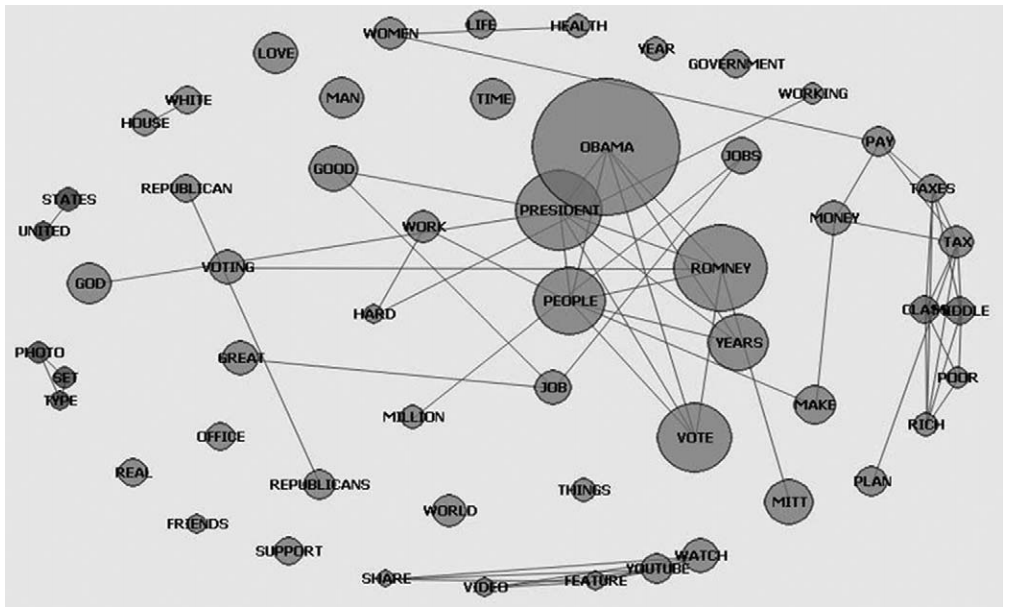
\includegraphics[scale=.75]{images/word_net.png} 
\caption{Barack Obaman sosiaalisen median sivuiden perusteella luotu kuva sanoista \citep{groshek2013public}}
\label{fig:wordnet}
\end{figure}

Laskennallisesti mielenkiintoisempaa on tekstin sisällön merkitysten arviointi, yksinkertaisimmillaan tekstin positiivisuuden ja negatiivisuuden arviointi. Jatkaen poliitikoiden sosiaalisen median tutkimusta, \citet{park2011networked} arvioivat poliitikkojen verkkoprofiilissa esiintyviä positiivisia je negatiivisia sanoja, ja havaitsevat että oppositiopuolueiden sivuilla oli enemmän positiivisia viestejä hallituspuolueisiin verrattuna. Myöskin \citet{tumasjan2010election} ovat kiinnostuneet poliitikkoihin liittyvistä viesteistä Twitterissä, he sentimenttianalyysin perusteella päättelevät, että puolueen kannattajat puhuvat kilpailevista poliitikoista negatiivisemmin kuin omasta ehdokkaastaan, mutta positiivisissa viesteissä ei nähdä selvää eroa.

Lisäksi laskennallisesti on mahdollista erottaa aiheita ja teemoja -- mikä vastaa ihmistyötä vastaavassa laadullisen tutkimuksen prosessissa. \citet{levy2013driving} ovat analysoineet lainsäädäntöön liittyneitä kommentteja ja laskennallisesti eroittaneet aineistosta teemoja, joita kommenteissa käsiteltiin. He analysoivat tarkemmin, ketkä ovat lähettäneet kommentteja ja havaitsevat eroja lobbausorganisaatioiden ja yksittäisten kansalaisten teemojen välillä. Tällä perusteella he arvioivat lainsäädäntötyön läpinäkyvyyttä ja lobbaustahojen merkittävyyttä lainsäädäntötyössä.

\subsection{Sentimenttianalyysi}

Esitellyissä artikkeleissa käytössä oli yksinkertainen, sanoihin ja niiden lukumäärään perustuva sentimenttianalyysi, jossa sanoja luokitellaan jollain asteikolla ja tätä kautta muodostetaan sanakirja, jota voidaan käyttää analysoimisessa \citep{pennebaker2001linguistic,Thelwall2010}\footnote{Sentimenttianalyysiä voidaan myös tehdä myös ohjaamattomasti, tavoite on aina löytää tekstiaineistosta piirteitä joiden perusteella voidaan ennustaa kielen käyttäytymistä. Käytettyjen menetelmien joukko on laaja, esimerkiksi Bayesilaisia luokittimia ja tukivektorikoneita on vertailtu \citep{Pang02a,Pang05a,Thelwall2010}. Koska sentimenttianalyysiä tutkitaan aktiivisesti, tässä työssä esittelen yksinkertaisen toteutuksen sentimenttianalyysistä.}. Analyysiä voidaan täydentää käyttämällä laajemmin kielellisiä ominaisuuksia, kuten huutomerkejä sekä perättäisille sanoja, sekä niiden vaikutusta yksittäisten termien määrään. On myös mahdollista koneellisesti testata erilaisia yhdistelmiä ominaisuuksia, ja verrata näin saatuja arvoja ihmisen suorittamaan luokitukseen lauseiden osalta, pyrkien optimoimaan eri ominaisuuksien painoarvoja siten, että virhe ihmisen tekemän luokituksen välillä on mahdollisimman pieni \citep{Thelwall2010}.

Sentimenttianalyysi perustuu siis tekstin piirteisiin \textit{(features)} tarkasteluun, laskennallisesti mielenkiintoisempi -- tosin, \citet{Thelwall2010}\footnote{\citet{Thelwall2010} on keskittynyt sosiaalisen median viestien analysointiin MySpace--palvelussa, ja samaa menetelmää on sovellettu myös löydetyssä kirjallisuudessa.} aineiston kohdalla vähemmän tarkka -- menetelmä on tukivektorikoneiden \textit{(support vector machine)} käyttö luokittamiseen. Tukivektorikoneita voidaan käyttää myös muuhun tekstuaalisen aineiston käsittelyyn \citep[esimerkiksi][]{Weber2012}.

Kyseessä on ohjatun oppimisen menetelmä, eli tukiverkkokoneet perustuvat piirrevektoreiden ja (opetettujen) arvojen pareihin. Olkoon siis aineistona $$\{ (x_1, y_1), (x_2, y_2), \ldots, (x_n, y_n) \}$$ missä $x_i \in \mathbb{R}^n$ on piirrevektori ja $y_i$ opetettu arvo $\in \mathbb{Z}$. Kyseessä on lineaarinen luokitin, joka siis jakaa piirreavaruus $X$ tasoilla, siten että arvot $y$ ovat mahdollisimman hyvin tasojen muodostamissa ryhmissä.

\begin{figure}
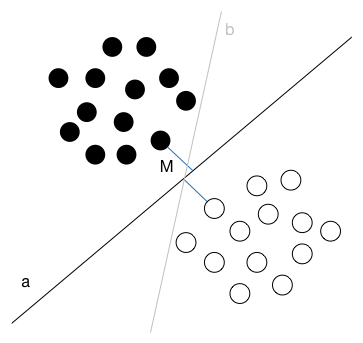
\includegraphics[height=5cm]{images/svm.png} 
\caption{Esimerkki tukivektorikoneen toiminnasta}
\label{fig:svm}
\end{figure}

Yksinkertaisuuden vuoksi oletamme tässä esityksessä, että $y_i \in \{ -1, 1 \}$i. Tukivektorikoneen tavoite on siis jakaa tämä joukko kahteen eri ryhmään yhdellä tasolla. Edelleen, tämän tason halutaan olevan sellainen, että alkioiden ja tason välinen etäisyys -- marginaali $M$ -- on mahdollisimman suuri, eli yksinkertaistetusti että löydetty taso jakaa aineiston mahdollisimman selvästi kahteen eri ryhmään. Tason määriytyy muutujien $\beta$ sekä $\beta_0$ avulla, jolloin tehtävänä on optimoida $\beta$n ja $\beta_0$ arvoja, siten että $M$ maksimoituu. Kuva \ref{fig:svm} esittelee ideaa tarkemmin: kahden joukon välissä oleva suora $a$ jakaa joukot siten, että marginaali $M$ on mahdollisimman iso. Vertaa sitä esimerkiksi vaihtoehtoiseen suoraan $b$, mikä sekin jakaa joukot kahteen ryhmään, mutta osa alkioista on erittäin lähellä tätä jakosuoraa.

Täsmällisesti siis, tavoite on määrittää $\beta$ ja $\beta_0$ luokittimessa sign$( x \beta + \beta_0)$. Edelleen, koska halutaan että ryhmien väliin jäävä marginaali $M$ on mahdollisimman iso. On siis tarkoitus löytää $\max M$ kuitenkin niin, että $y_i( x_i \beta + \beta_0 ) \geq M - \varepsilon$. $\varepsilon$ on lisätty yhtälöön sallimaan osan alkioista olemaan marginaalin sisällä, yksinkertaisuuden vuoksi tässä esityksessä $\varepsilon = 0$.

Yllä kuvattu optimointiongelma voidaan myös esittää muodossa $$ \min \frac{1}{2} || \beta ||^2 $$, kuitenkin huomioiden että $ y_i( \beta x_i + \beta_0 ) \geq 1$. Ongelmaan voidaan soveltaa neliöllistä optimointia, jolla ratkaistaan pienin mahdollinen $\beta$n arvo. Jos oletamme, että $\varepsilon \neq 0$, ongelmaan  sovelletaan Lagrangen menetelmää, edelleen jos jakoa ei suoriteta lineaariluokittimella on tarpeen siirtyä käyttämään kernelifunktiota \citep{vapnik1982estimation,cortes95,Hastie2009}.

\subsection{Teemojen luokittelu}

Teemojen luokittelussa syötteenä on joukko teksidokumenteja $D_1, D_2, \ldots, D_n$ ja tavoitteena on eritellä mistä teemoista $t_1, t_2, \ldots, t_m$ kyseiset dokumentit käsittelivät. Kyseessä on ohjaalamttoman koneoppimisen muoto, eli aiheita ei tarvitse etukäteen määritellä -- ja mikä tärkeintä, ei ole tarpeen yhdistää dokumentteja ja aiheita opetusaineiston luomiseksi. Ratkaisu perustuu kunkin tekstidokumentin sanojen ja niiden todennäköisyyksien analysoimiseen.

Menetelmänä teemojen luokittelussa voidaan käyttä latenttien Dirchlet-allokaatioihin \textit{(latent Dirchlet allocation, LDA)} perustuva todennäköisyyslaskenta. Ideana on siis, että aineistolla on piilossa olevia teemoja, joita voidaan havainnoida välillisesti sanojen esiintymisen perusteella dokumenteissa \citep{Blei2010,Blei2003}.

\subsection*{Työkalut}

Agenttipohjaisten simulaatioiden kohdalla korostettiin dokumentaatiota, avoimuutta ja muokattavuutta eri ympäristöjen arvioinnissa \citep{Tobias2004}. Sentimenttianalyysissä samanlaiset kriteerit ovat mielekkäitä: kuitenkin, koneoppimista soveltavissa lähestymistavoissa mielekästä on myös arvioida koneopitun aineiston laatua ja luotettavuutta. Esimerkiksi \citet{Thelwall2010} kehittämä SentiStrength tarjoaa valmiina käytettäväksi englannin kielelle soveltuvan sanakirjan, mutta mahdollistaa myös omien painotusten kehittämisen ja optimoinnin.

Sekä tukivektorikoneisiin että teemojen luokitteluun löytyy useita avoimen lähdekoodin toteutuksia. Koska kyseessä on olemassa olevien menetelmien laskennalliset toteutukset, on mielekästä tarjota niistä  \citet{hornik2006support} esittelevät neljän erilaisen tukivektorikoneita käsittelevää kirjastoa, ja päätyvät suosittelemaan suorituskykynsä puolesta \texttt{kernlab}-pakettia sekä \texttt{e1071}-paketissa olevaa, libsvm-kirjastoon perustuvaa toteutusta. Myös aiheiden tunnistukseen on olemassa R-paketti \texttt{topicmodels}.

\section{Säännönmukaisuuksien ja ryhmien löytäminen}
\label{unsupervised}

Viimeisenä laskennallisten menetelmien ryhmänä esittelen ohjaamattoman oppimisen menetelmiä, jotka pyrkivät löytämään säännönmukaisuuksia numeerisesta aineistosta. Esimerkiksi politiikan tutkimuksen perinteinen teema on selittää eroja valtioiden välillä, esimerkiksi demokratian tilan arviointia taustamuuttujien perusteella. \citet{Jurek2013} jatkavat tätä perinteistä linjaa selittämällä valtioiden demokaattisuutta Freedom House --aineiston ja taustamuuttujien, kuten uskonnon ja demokratian keston perusteella. Menetelmänä he käyttävät työssään assosiaatiosääntöjen hakua laskennallisesti, jonka perusteella he löysivät yhteensä 210 erilaista sääntöä. Lisäksi he nostavat esille, että koneoppimisen soveltaminen mahdollistaa selittävien tekijöiden muutoksien valitsemisen vapaammin kuin perinteisten tilastollisten mentelmien soveltaminen, jossa tarkasteltavien sääntöjen määrä on yleisesti merkittävästi pienempi.

Muita ohjaamattoman oppimisen menetelmiä on muuttujien dimensioiden vähentäminen (\textit{dimensionality reduction}), pääkomponenttianalyysi sekä klusterointianalyysi \citet[485--586]{Hastie2009}. Dimensioiden vähentäminen esimerkiksi pääkomponenttianalyysin avulla on yleisesti tiedossa oleva menetelmä jo nyt \citep[esimerkiksi][615--651]{metsamuuronen}, mutta klusterointimenetelmistä $k-means$--mentetelmä on toistaiseksi tuntemattomampi politiikan tutkimuksen piirissä.

%% Marketing Segmentation Through Machine Learning Models An Approach Based on Customer Relationship Management and Customer Profitability Accounting

%% Kaufman and Rousseeuw (1990)

%% Ohjaamatonta koneoppimista voi lähestyä useilla erilaisilla menetelmillä, kuten assosiaatiosäännöillä, dimensioiden vähentämisellä (\textit{dimensionality reduction}) sekä  klusteroimalla \citet[485--586]{Hastie2009}\footnote{\citet[43--138]{Hastie2009} nostavat myös regressiomallit koneoppimisen osana, mutta kuten johdannossa argumentoin kyseessä on yhteiskuntatieteen näkökulmasta enemmänkin perinteinen laskennallinen menetelmä, enkä siksi esittele tarkemmin näiden yksinkertaisten mallien käyttöä osana laskennallista yhteiskuntatiedettä.}. \todo{Lisää johdattelua?}

\subsection{Assosiaatiosäännöt}

Assosisaatiosäännöt perustuvat aineiston ominaisuuksien $x_1, x_2, \ldots, x_n$ perustuvat, että voidaan löytää yhteyksiä ominaisuuksien välillä. Yleisesti ominaisuudet ovat binäärisiä, eli $x_i \in \{ 0, 1\}$. Tavoitteena on löytää sääntöjä muuttujien välisistä suhteista: esimerkiksi $(x_h, x_i, x_j) \Rightarrow x_k$. Sääntöjen määrä kasvaa $2^n$-nopeudella, jolloin haaste on löytää säännöistä mielenkiintoiset, kattavat ja luotettavat säännöt. Jotta tämä ongelma olisi ratkaistavissa, kustakin säännöstä lasketaan erikseen sen selitysaste, luottamus kyseisen säännön yleistettävyyteen ja säännön nosto (\textit{lift}), jolla arvioidaan löydetyn säännön merkittävyyttä \citep[485--586]{Hastie2009}.

Eräs algoritmi kattavien muodostamiseksi on \citet{Agrawal1994a} esittelemä Apriori. Kuten algoritmi \ref{algo:apriori} näyttää, Apriori laskee eri sääntökombinaatioiden esiitymisen aineistosta ja riippuen vaaditusta tuesta joko hyväksyy sääntökombinaation osaksi kattavia sääntöjä tai hylkää sen. Uudet sääntöehdokkaat luodaan yksinkertaisesti käymällä aiemmat $n$ alkion kokoisten sääntöjen joukko läpi ja lisäämällä siihen mahdollinen $n+1$ pituisen sääntöjen joukko, kunnes $n+1$ pituisia mahdollisia sääntöjä ei enää ole.

\begin{algorithm}
\begin{algorithmic}
\State Olkoon $\mathcal{S}$ kaikki aineistossa esiintyvät siirtymät, eli kaikki aineiston rivit [$x1, x2, \ldots, x_m$]
\State Olkoon $\varepsilon$ vaadittu vähimmäistuki mielenkiintoisena pitämiseen

\State $S_1 \gets $ \{ kaikki yhden alkion kokoiset säännöt \}
\State $i \gets 2$

\While{ $S_{i-1} \neq \emptyset$ }

  \State $E_i \gets \{ a \cup \{b\} \mid a \in S_{k-1} \land b \in \bigcup S_{k-1} \land b \not \in a \} $

	\ForAll{$s in \mathcal{S}$}
	    \ForAll{ehdokas $\in \{ e | e \in E_i \land e \subseteq \mathcal{s} \}$}
		   \State $e$.maara $ \gets + 1$
		\EndFor

	\EndFor 

		\State $S_i \gets \{ e | e \in E_i \land e.\mathrm{maara} \geq \varepsilon \}$
		\State $i \gets +1$
\EndWhile

\Return $\bigcup_i S_i$
\end{algorithmic}
\caption{Apriori-algoritmi}
\label{algo:apriori}
\end{algorithm}

Algoritmin jälkeen kerättynä on siis kattavat joukot, joista on tarpeen valita edelleen luotettavat ja mielenkiintoiset säännöt. Tätä varten määritellään säännön $X$ tuki todennäköisyytenä, että aineistosta löytyy sekä ryhmä $X$, missä $X \subset \{ x_1, x_2, \ldots , x_n \}$. Luottamus sääntöön määritellään tuen avulla, ja se normalisoi säännön esiintyvyyden suhteessa mahdollisiin esiintymisiin: luottamus($A \Rightarrow B) = \frac{\mathrm{tuki}(A \union B)}{\mathrm{tuki}(A)}$, jälleen $A,B \subset \{ x_1, x_2, \ldots , x_n \}$. Intuitiivisesti siis, jos aineistossa on paljon $A$ta, niin tällöin luotettavan säännön muodostamiseksi tarvitaan vahva evidenssi parista $(A,B)$, vastaavasti jos aineistossa on vähän $A$ta, ei paria $(A,B)$ vaadita niin useita. Kattavista joukoista lasketaan luottamus ja valinnaisen kynnyksen perusteella säännöistä epäluotettavat hylätään ja luotettavat jätetään käsittelyyn.

\subsection{Klusterointi}

Dimensioiden vähentämisellä viitataan prosessiin, jossa ilmiötä kuvaavien muuttujien määrää vähennetään etsimällä muuttujaryhmiä, joiden kautta aineiston vaihtelua selitetään mahdollisimman hyvin. Yhteiskuntatietelijöiden yleisesti tuntema menetelmä tähän on pääkomponenttianalyysi (\textit{principal component analysysi, PCA}), jonka kautta aineisto jaetaan selittäviin faktoreihin. Laskennalliset menetelmät mahdollistavat myös aineiston samankaltaisten alkioiden esittämisen ryhminä, eli klustereina. Ongelmana siis muotoillaan seuraavasti: joukko alkioita $\{ x_1, x_2, \ldots, x_n \}$ halutaan jakaa $k$hon ryhmään, siten että nämä ryhmät edustavat aineiston piirteitä.

\citet{llyod1982} esittämä ratkaisu ongelmaan on $k$-means-algoritmi: se löytää aina lokaalisti parhaan ratkaisun ongelmaan (\textit{local minimum}), mutta ei takaa että tämä ratkaisu on yleisesti paras (\textit{global minimum}). Globaalisti parhaan ratkaisun löytäminen on kuitenkin laskennallisesti vaativa, jolloin sovelluksissa tyydytään heuristiseen lokaalisti parhaaseen ratkaisuun.

Nimensä mukaisesti $k$-means löytämään keskiarvon kullekkin klusterille ja valitsemaan klustereiden sijainnit siten, että havaintojen sijoittaminen näille klusteripisteille minimoi neliöllisen virheen (Algoritmi \ref{algo:kmeans}). Yksinkertaisuuden vuoksi oletamme, että $x_i \in \mathbb{R}^n$, jolloin vektorien välisiä etäisyyksiä voidaan laskea selkeästi; $k$-means menetelmä on toki yleistettävissä yleiselle etäisyysfunktiolle $\mathcal{D}(a,b)$. Täsmällisemmin siis minimoidaan $\sum_i ||x_i - k_{x_i}||^2$, missä $k_{x_i}$ on alkiota $x_i$ vastaava klusteri. Kyseessä on iteratiivinen algoritmi, jota toistetaan kunnes klustereiden sijainnit eivät vaihdu.

Vastaavasti spektriklusterointi perustuu samankaltaisten ominaisarvojen ryhmittämistä, jolloin klusterit korostavat samankaltaisten ominaisuuksien joukkoja paremmin kuin keskiarvoon perustuva $k$-means klusterointi \citep[485--586]{Hastie2009}.

\begin{algorithm}
\begin{algorithmic}

\State Jaetaan aineisto alustavasti klusteriryhmiin $k_1, k_2, \ldots k_k$ ja etsitään jokaiselle alkiolle $e$ alkiota lähinnä oleva klusteri

\While{klusterien paikat eivät merkittävästi muutu}

\State lasketaan jokaiselle klusterille $k$ uusi paikka $k'$ laskemalla keskiarvo klusteriin kuuluvien alkioiden $x_{1}, x_{2}, \ldots x_{m}$ paikoista, eli $k' = \frac{1}{m} \sum_{i=1}^m x_i $
\State uudelleenmääritellään alkoiden kuuluminen klusteriryhmiin tarkastamalla, mitä klusteria $k'_i$ lähinnä alkio $x$ on, eli $\min_{i=1}^k || x - k'_i || ^ 2$

\EndWhile

\end{algorithmic}
\caption{k-means-algoritmi}
\label{algo:kmeans}
\end{algorithm}


\section{Keskustelu}

\subsection{Validiteetti haasteena}

Niin määrällisessä kuin laadullisessa yhteiskuntatieteessä tutkimuksen laatua arvioidaan validiteetin ja reliabiliteetin kannalta. Ensimmäinen viittaa ulkoiseen laatuun, eli siihen tutkitaanko ilmiötä oikein ja jälkimmäinen sisäiseen laatuun, eli onko tutkimus tehty uskottavasti.

Sentimenttianalyysi, teemojen luokittelu, assosiaatiosääntöjen oppiminen sekä klusterointi ovat aineiston käsittelyyn tarkoitettuja algoritmeja, jolloin uskottavuuden kannalta keskeisempää on aineiston laatu: onko aineiston mahdollinen esikäsittely suoritettu oikein ja onko aineisto kerätty oikein. Iteratiivissa algoritmeissa -- kuten klusteroinnissa -- on tarpeen myös tarkastella tulosten pysyvyyttä eri aloitusarvoilla, eli arvioida saadun tuloksen herkkyyttä \todo{two-solution-problem paperi EDMStä?}. Käsitellessään tutkimuksen laadukkuutta, \citet{Grimmer2013} huomioivat, että laskennallisten menetelmien käytön tulisi vastata ihmisten tekemän analyysin tasoa, eli taustateorioiden, käsin tehdyn aineiston käsittelyn tai tilastollisten arvioiden tulee luoda luottamus menetelmien uskottavuudesta ja sopivuudesta ongelmaan.

Kirjallisuuden pohjalta laskennallisen yhteiskuntatieteen käytetyn menetelmä oli simulointi, joka on mielestäni uskottavuuden kannalta myös haastavin. Toisin kuin yllä mainituissa menetelmissä, simuloinnissa menetelmä ja käytettyjen parametrien määrä voi vaikuttaa tulokseen. \citet{bloomquist2006comparison} on työssään arvioinut kolmea julkaistua agenttipohjaista mallia, havaiten ettei tuloksia näissä malleissa ole verrattu ilmiöstä kerättyyn aitoon aineistoon. Lisäksi  hän kritisoi sitä, ettei malleilla ole suoritettu useampia ajoja, jolloin mallien tuloksiin liittyy tiettyä epävarmuutta. Samoin \citet{edmonds2005computational} arvioivat erilaisia simulointimalleja, nostaen esille huolensa toistettavuudesta sekä ymmärryksen mallin rajoituksista ja soveltuvuudesta eri teemoihin.

Kritiikki on mielestäni osuvaa ja osoittaakin suurimman huoleni simulaatiotutkimukseen: kuinka voidaan varmistaa, että esitetyt simulaatiot aidosti vastaavat varsin monimutkaisia yhteisöjen käyttäytymissääntöjä? Viimeaikaisessa simulaatiotutkimuksessa näihin kritiikkeihin on pyritty vastaamaan, esimerkiksi simulaatiomalli voidaan rakentaa ilmiötä tutkivien koeasetelmien valossa \citep{Villatoro2013} tai mallien tuloksia voidaan verrata olemassa oleviin ilmiöihin aktiivisesti ja käyttää näitä mallin rakennuksen tukena \citep{Pearson2011}.

Simulaatiomallit heikkouksistaan huolimatta tarjoavat kiinnostavia mahdollisuuksia mallin luomiseen vuorovaikutuksessa laskennallisten sekä yhteiskuntatieteilijöiden ja muiden toimijoiden välillä. \citet{Milne2014} kuvaavat prosessia, jossa simulaatiomallia ja sen tuloksia arvioitiin yhdessä virkamiesten ja tutkijoiden välillä. Heidän mukaansa mahdollisuus muuttaa mallia lisäsi yhteisymmärrystä ilmiöstä ja helpotti tiedon siirtämistä tutkijoilta soveltajille. Toisaalta, kuten \citet{Saunders-Newton2001a} huomauttavat, eri henkilöt suhtautuvat laskennallisiin menetelmiin myös erilaisin odotuksin. Tällöin luottamuksen rakentaminen ja laskennallisen menetelmän läpinäkyvyys ja selkeys ovat merkittäviä arvoja osana laskennallista yhteiskuntatiedettä, kuten perinteisessä yhteiskuntatieteellisessä tutkimuksessa.

\subsection{Työskentely monitieteellisesti}

\begin{figure}

%\begin{subfigure}{.6\textwidth}
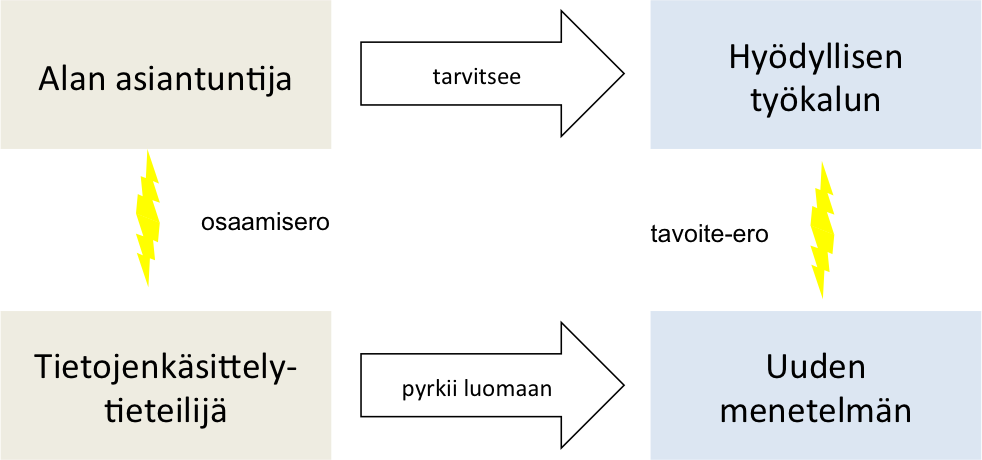
\includegraphics[width=.6\textwidth]{images/monitieteellisyys_ongelma.png} 
\caption{Menetelmäkehityksen ero soveltajaan \citep[mukaillen][7]{Wijk2006}}
\label{fig:domain_expert_vs_computation_specialist}
%\end{subfigure}
%~~
%\begin{subfigure}{.2\textwidth}
%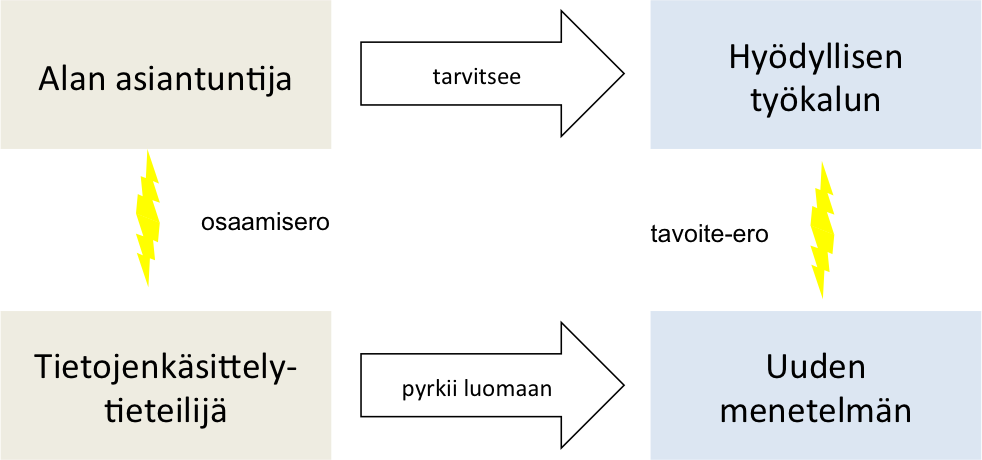
\includegraphics[width=\textwidth]{images/monitieteellisyys_ongelma.png} 
%\caption{Menetelmäkehityksen ero soveltajaan \citep[mukaillen][7]{Wijk2006}}
%\end{subfigure}

\end{figure}

Tutkimuksen uskottavuuden kohdalla nostin esille jo haasteen yhteistyöstä laskennallisen ja yhteiskuntatieteen välillä. \citet{Wijk2006} käsittelee monitieteellistä yhteistyötä visualisoinnissa. Oman kokemuksensa pohjalta hän huomauttaa, että alan asiantuntijalla (\textit{domain expert}) ja visualisaation tutkijalla on usein erilaiset tavoitteet visualisaation kehittämisessä: kun visulisaation tutkija ensisijaisesti kehittää uusia visualisaatiomenetelmiä, niin alan asiantuntijan tavoitteena on hyödyllisen työkalun kehittäminen -- mikä voidaan saavuttaa myös perinteisillä menetelmillä. Kuvassa \ref{fig:domain_expert_vs_computation_specialist} esitän saman erottelun sovellettuna laskennalliseen yhteiskuntatieteeseen, alan asiantuntijan ja tietojenkäsittelytietelijöiden välisenä tarkasteluna.

\citet{Wijk2006} jatkaa, että tavoite-eron takia yhteistyön muoto on joku seuraavista: tietojenkäsittelytieteen asiantuntija voi hänen mukaansa toimia työvälinekehittäjänä tai jatkaa tietojenkäsittelyn menetelmien kehittämistä. Tietojenkäsittelytieteen asiantuntija voi myös soveltaa käyttäjäkeskeisiä menetelmiä kehitystyössään, jolloin laskennallisia menetelmiä kehitetään yhteistyössä alan asiantuntijan kanssa. Toisaalta, tietojenkäsittelyttieteen asiantuntija voi myös itse tutustua alaan tai kehittää visualisaatiotekniikoita aiheisiin, joista hän on kiinnostunut. van Wijk kutsuu viimeistä yhteistyön muotoa mielenkiintovetoiseksi kehitystavaksi (\textit{curiosity driven}), ja nostaa esille muodon haasteen: sellaisenaan tällä toimintatavalla ei voida ratkaista aihealueen haastavimpia ongelmia.

Laskennallisen yhteiskuntatieteen osalta merkittävä kysymys onkin, kuinka yhteistyötä tietojenkäsittelytieteen ja yhteiskuntatieteen välillä voitaisiin parantaa, jolloin aineiston analysoimiseksi olisi käytössä tehokkaat ja uskottavat teknologiat. Eräs keino olisi soveltaa käyttäjäkeskeisen suunnittelun \textit{(user-centered design, UCD)} periaatteita yhteistyöprojekteissa: soveltajan tarpeita ja tutkimustraditioita pyritään ymmärtämään laaja-alaisesti ja tukemaan tutkimustradition mukaista toimintaa. Tällöin kuitenkin haasteena on nimenomaisesti ottaa huomioon myös tietojenkäsittelytieteen tutkimuksen kannalta mielekkäät kysymykset osana tutkimusta.

Vaihtoehtoisesti laskennallinen yhteiskuntatiede voidaan tulkita menetelmäkehityksen kannalta vähemmän oleelliseksi alaksi: laskennalliset menetelmät kehittyvät tietojenkäsittelytieteen tutkijoiden joukossa ja joskus osa näistä menetelmistä siirtyvät käyttöön soveltajien -- kuten yhteiskuntatietelijöiden -- joukkoon.

\subsection{Paradigman muutos?}

Mikä merkitys laskennallisella yhteiskuntatieteellä on? \citet[265]{watts11} argumentoi, että

\begin{quote}
\texttt{[o]}n kuitenkin välttämätöntä soveltaa kaikkia näitä \texttt{[sekä laskennallisia että kuvailevia]} lähetymistapoja samanaikaisesti, pyrkien saavuttamaan johtopäätöksiä siitä, kuinka ihmiset käyttäytyvät ja kuinka maailma toimii -- sekä ylhäältä että alhaalta, käyttäen hyödyksi kaikkia menetelmiä jotka ovat käytettävissä. (\textit{oma suomennus})
\end{quote}

Laskennallisille menetelmille yhteiskuntatieteissä on siis tarvetta, koska niiden avulla on mahdollista esittää ratkaisuja uusiin kysymyksiin. Kuitenkin, samaan aikaan tulee huomioida yhteiskuntatieteiden oppihistoria monimenetelmäisenä ja -paradigmaisena: eri lähestymistapojen käyttö samojen ongelmien käsittelyyn on perinteinen menetelmä yhteiskuntatieteiden osalta.

Kirjallisuuskatsauksen perusteella laskennallisen menetelmät ovat toistaiseksi selkeästi vähemmistössä julkaistujen artikkelien joukossa. Kuitenkin laskennalliset menetelmät tarjoavat kiinnostavia mahdollisuuksia aineistojen, niin määrällisten kuin laadullisten, tarkasteluun ja esikäsittelyyn tutkimusta tukien. En usko laskennallisten menetelmien muuttavan merkittävästi yhteiskuntatieteen tapaa toimia, vaan kehittävän eteenpäin jo nyt vakiintuneita empiirisen tutkimuksen menetelmiä.

\section{Johtopäätökset}

Työssä käsiteltiin laskennallisia menetelmiä yhteiskuntatieteiden toiminnassa, ja tätä kautta muodostunutta laskennallisen yhteiskuntatieteen toimikenttää. Työn ensimmäinen kontribuutio käsittelee toimintakentän määritelmää: laskennalliselle yhteiskuntatieteelle ei löydy yksikäsitteistä määritelmää ja alan konfferensseissa esitellään esimerkiksi taideprojekteja. Onkin mielekästä puhua laskennallisen yhteiskuntatieteen jatkumosta, jossa laskennallisten menetelmien monimutkaisuus vaihtelee.

Kirjallisuuskatsauksen perusteella suurimmaksi laskennallisuuden sovellusalue on simulaatiotutkimuksessa, erityisesti agenttipohjaisessa simulaaatiossa. Ohjatut ja ohjaamattomat koneoppimisen menetelmät tarjoavat mielenkiintoisia mahdollisuuksia, mutta niiden käyttö ei ole vielä vakiintunut vertailuissa journaaleissa tarkemmin. Yhteiskuntatieteellisissä julkaisuissa on kuitenkin sovellettu esimerkiksi aiheiden tunnistamista, sentimenttianalyysiä ja assosiaatiosääntöjä koneoppimisen menetelminä.

Kirjallisuuskatsauksen perusteella laskennallisella yhteiskuntatieteellä on kaksi merkittävää haastetta: tutkimuksen luotettavuus ja poikkitieteellinen yhteistyö. Tutkimuksen luotettavuuteen ei ole yksikäsitteistä ohjetta, vaan käytössä on esimerkiksi koeasetelmien kautta saavutettu luottamus malleihin \citep{Villatoro2013}, aktiivinen vertailu olemassa oleviin tilastotietoihin \citep{Pearson2011} sekä saman tutkimusprosessin toistaminen ainakin osittain perinteisin menetelmin \citep{edmonds2005computational}. Myös ryhmätyöskentelyn rooli osana tutkimuksentekoprosessia on nostettu esille validiteettia parantavana tekijänä \citep{Milne2014}, mikä myös voi olla ratkaisu poikkitieteellisen työskentelyn haasteisiin.

\section*{Kiitokset}

Kiitän työn ohjaajaa, Antti Ukkosta, keskusteluista ja kyseenalaistavista kysymyksistä. Lisäksi kiitän Airi Lampista sekä Eric Malmia työn aikana käydyistä keskusteluista.


\newpage

\bibliographystyle{abbrvnat}
\addcontentsline{toc}{section}{Lähteet}
\bibliography{bsc,/Users/mnelimar/Dropbox/_tools/library.bib} 

\newpage

\appendix

\section{RePast-esimerkki}
\label{appedix:repast}

\lstinputlisting[language=Java,breaklines=true,numbers=left,tabsize=1]{examples/RePast.java} 

RePast-dokumentaation pohjalta luotu esimerkki.

%% http://repast.sourceforge.net/docs/RepastJavaGettingStarted.pdf

\end{document}
